\chapter{Modelagem matemática}

\section{Modelagem matemática}

Dentro da pesquisa, foram realizadas duas modelagens distintas, ambas, diferentemente da literatura clássica, foram elaboradas com base nas estações de origem e destino, e não nos legs do percurso.

Para compreender essas propostas, consideremos uma versão simplificada do problema como se mostra na figura \ref{fig: fig1}, onde temos:

\begin{itemize}
	\item 4 estações pelas quais o trem deve passar em um único sentido, ou seja, o trem não tem retorno.
	\item O trem tem uma capacidade máxima de assentos.
	\item Há apenas um tipo de classe comercial.
	\item Existe apenas um período no horizonte de reserva.
	\item A variável de decisão é a quantidade de assentos que pode ser disponibilizada para venda em um trecho com origem e destino específicos.
	\item Todos os assentos disponibilizados para venda serão vendidos.
\end{itemize}

\begin{figure}[th]
	\begin{center}
		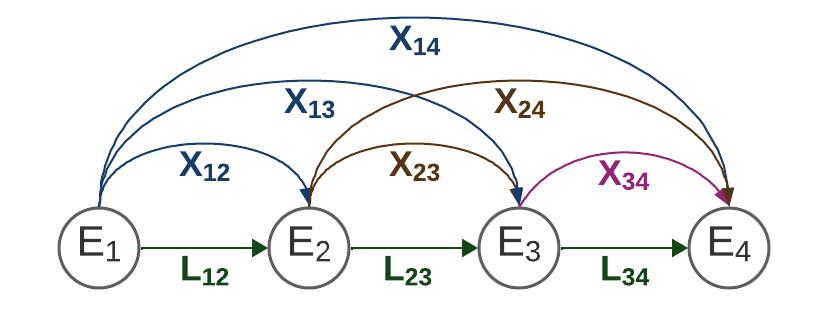
\includegraphics[scale=0.7]{img/fig1.png}
		\caption{Versão gráfica simples}
		% Fonte:~\cite{khaksar2013genetic}}
		\label{fig: fig1}
	\end{center}
\end{figure}


\section{Primeira modelagem matemática}\label{sec:modelo1}

Agora, para a primeira proposta de modelagem, temos o seguinte

\noindent $x_{ij}$: Quantidade de assentos que será disponibilizada para venda no trecho com origem em $i$ e destino em $j$, onde $j>i$ \\
\noindent $A_i$: Disponibilidade do trem na estação $i$ \\
\noindent $P_{ij}$: Preço da passagem no trajeto com origem em $i$ e destino em $j$ \\
\noindent $Q$: Capacidade do trem

Dado o exposto, a função objetivo será maximizar o lucro para cada possível venda em cada trajeto $i,j$, matematicamente seria:

$FO: max \quad x_{12}P_{12} + x_{13}P_{13} + x_{14}P_{14} + x_{23}P_{23} + x_{24}P_{24} + x_{34}P_{34}$

s.a.

Estação 1: $x_{12} + x_{13} + x_{14} \leq A_1 \quad onde \quad A_1 = Q $ \\
\indent Estação 2: $x_{23} + x_{24}  \leq  A_2 \quad onde \quad A_2 = A_1 - (x_{12} + x_{13} + x_{14}) + x_{12} $ \\ 
\indent Estação 3: $x_{34} \leq A_3 \quad onde \quad A_3 = A_2 - (x_{23} + x_{24}) + x_{13} + x_{23} $

Note que as restrições são aplicadas para cada uma das três primeiras estações, E1, E2 e E3, já que são as estações que têm pelo menos um destino, e a última estação, E4, é excluída, pois não possui nenhum destino.

Cada uma das restrições leva em consideração o fluxo de pessoas que sairão e entrarão no trem. Levando isso em conta, é necessário calcular a disponibilidade do trem para cada estação. Considere uma solução viável para o modelo, conforme mostrado na figura \ref{fig: fig2}, com uma capacidade total de 100 assentos para um trem.

\begin{figure}[!ht]
	\begin{center}
		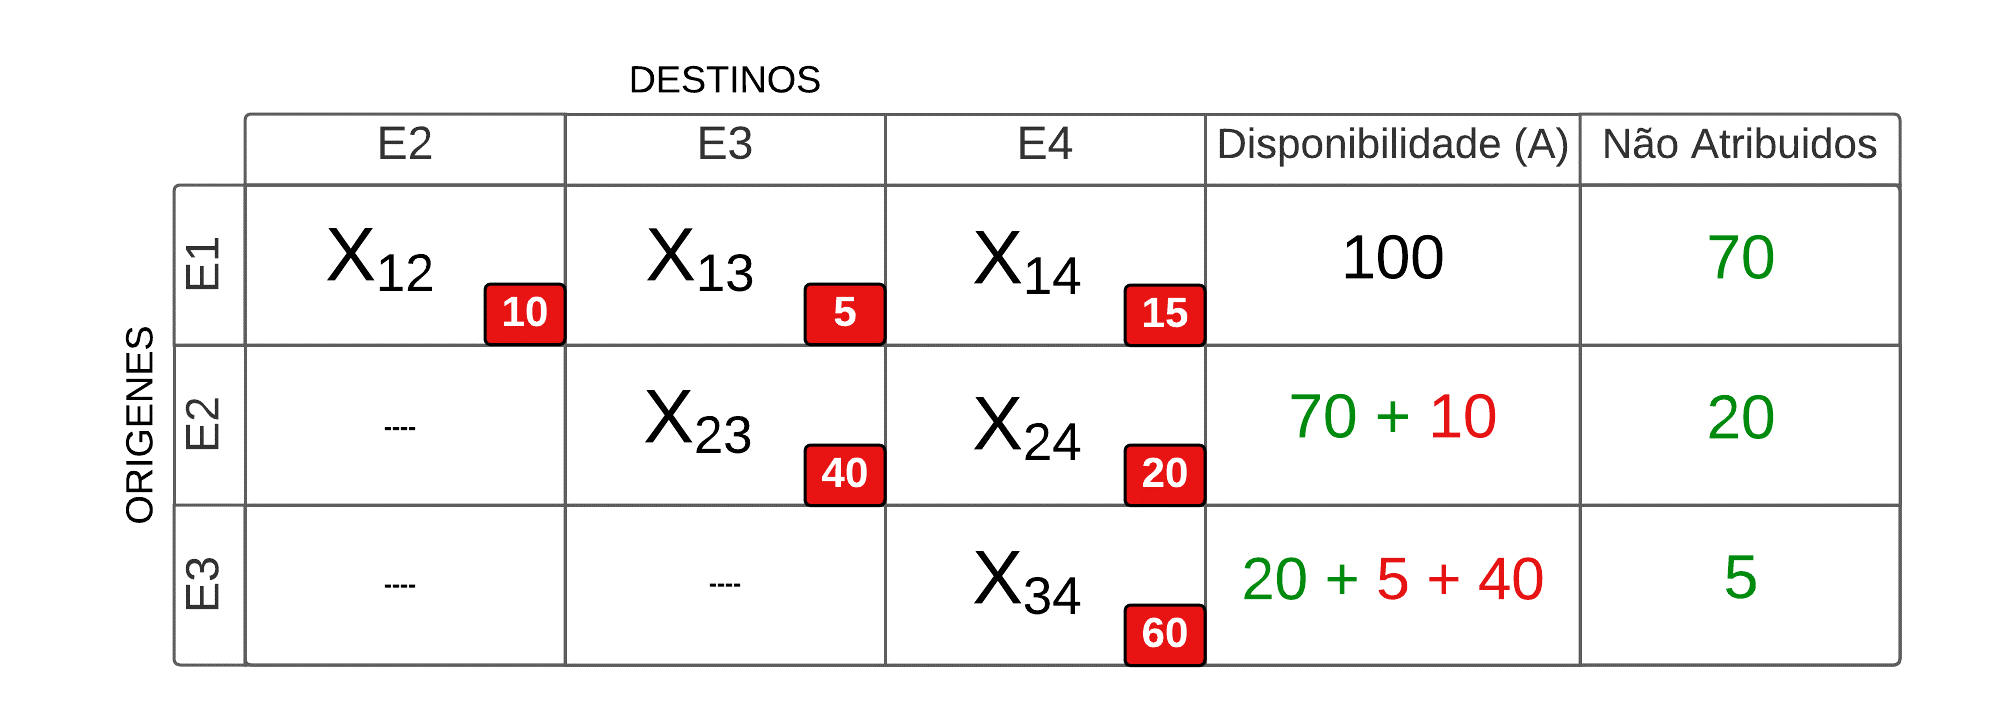
\includegraphics[scale=0.4]{img/fig2.png}
		\caption{Solução factível para o problema simplificado}
		% Fonte:~\cite{khaksar2013genetic}}
		\label{fig: fig2}
	\end{center}
\end{figure}

Note que, para a restrição da estação 1, o trem está com todos os assentos vazios, ou seja, \(A_1=100\), e que a soma das variáveis seria \(x_{12} + x_{13} + x_{14} = 10 + 5 + 15 = 30\). Portanto, teríamos \(30 \leq 100\), ou seja, foram disponibilizados para venda 30 assentos dos 100 que o trem possui. Nesse sentido, no momento da partida do trem da estação 1, haveria 70 assentos vazios ou disponíveis para venda em estações posteriores.

Agora, para a estação 2, teríamos \(A_2 = 100 - 30 + 10 = 70 + 10 = 80\). Já era conhecido que havia 70 assentos disponíveis vindos da estação 1, mas também é preciso levar em conta que os assentos com destino à estação 2 também ficarão disponíveis da estação 2 em diante, para este caso \(x_{12} = 10\). Portanto, para a estação 2, teríamos 80 assentos vazios para disponibilizar, ou seja, \(60 \leq 80\). Analogamente, o mesmo raciocínio seria aplicado para a estação 3, ou seja, teríamos a soma de todos os assentos que chegaram à estação 3, \(x_{13} = 5\) e \(x_{23} = 40\), assim teríamos \(A_3 = 80 - 60 + 5 + 40 = 20 + 5 + 40 = 65\), e no final teríamos \(60 \leq 65\).

Dada a lógica anterior, vejamos agora o modelo proposto completo:

\begin{table}[h]
	\centering
	\small
	\begin{tabular}{p{2cm} p{9.5cm} p{3.2cm}}
		\toprule
		\textbf{Definição} & \textbf{Notação}                                                                     & \textbf{Domínio}                     \\ \midrule
		\multicolumn{3}{l}{\textbf{Conjuntos}}                                                                                                           \\ \midrule
		I                  & Conjunto de estações de Inicio                                                       &                                      \\
		J                  & Conjunto de estações de Destino                                                      &                                      \\
		K                  & Conjunto de Classes de Control                                                       &                                      \\
		T                  & Conjunto de Check-Points (Períodos)                                                  &                                      \\ \midrule
		\multicolumn{3}{l}{\textbf{Parâmetros}}                                                                                                          \\ \midrule
		n                  & Quantidade de estações                                                               &                                      \\
		Q                  & Capacidade do trem                                                                   &                                      \\
		P$_{ijk}$          & Preços  dos passagem com origem i, destino j e classe de control k                   & $i \in I, j \in J, k \in K$          \\
		D$_{ijkt}$         & Demanda  de passagem com origem i, destino j e classe de control k                   & $i \in I, j \in J, k \in K, t \in T$ \\ \midrule
		\multicolumn{3}{l}{\textbf{Variáveis de decisão}}                                                                                                \\ \midrule
		A$_{i}$            & Disponibilidade de passagens para vendas na estação i                                & $i \in I$                            \\
		X$_{ijkt}$         & Quantidade de passagem atribuídos no tramo i,j com classe de control k no período t  & $i \in I, j \in J, k \in K, t \in T$ \\
		Y$_{ijkt}$         & Quantidade de passagem autorizados no tramo i,j com classe de control k no período t & $i \in I, j \in J, k \in K, t \in T$ \\ \bottomrule
	\end{tabular}
	\caption{Notação matemática}
	\label{Notacao}
\end{table}

\begin{eqnarray}
	&& Max \quad Z = \sum_{i\in I} \sum_{j\in J} \sum_{k\in K} \sum_{t\in T} P_{ijk} X_{ijkt} \label{eq: m1_ecu1}                                                                    \\
	&& \text{s.a.}  \notag                                                                                                                                                    \\
	&& A_{i} = A_{i-1} - \sum_{j\in J/j \geq i}\sum_{k\in K}\sum_{t\in T}X_{i-1,j,k,t} + \sum_{j\in J /j<i}\sum_{k\in K}\sum_{t\in T}X_{jikt}, \quad \forall i  \label{eq: m1_ecu2}  \\
	&& \sum_{j \in J}\sum_{k\in K}\sum_{t\in T} X_{ijkt} \leq A_{i} , \quad \forall i/i<j, i < n                                                \label{eq: m1_ecu3}                  
\end{eqnarray}
\begin{eqnarray}
	&& Y_{ijkt} \geq X_{ijkt},  \quad \forall i,j,k,t/ i < j                                                                          \label{eq: m1_ecu4}                            \\
	&& Y_{ijkt} \leq Y_{i,j,k+1,t},  \quad \forall i,j,k,t / i < j, k < \lVert K \rVert,  P_{ijk} \leq P_{i,j,k+1}                      \label{eq: m1_ecu5}                          \\
	&& X_{ijkt} \leq D_{ijkt},  \quad \forall i,j,k,t/ i < j                                                                           \label{eq: m1_ecu6}                           \\[15pt]
	&& X_{0,j,k,t} = 0,     \quad \forall j,k,t                                                                                        \label{eq: m1_ecu7}                           \\
	&& A_{0} = Q                                                                                                                      \label{eq: m1_ecu8}                            \\
	&& X_{ijkt} \in \mathbb{Z}^+                                                                                                   \label{eq: m1_ecu9}                               \\
	&& Y_{ijkt} \in \mathbb{Z}^+                                                                                                   \label{eq: m1_ecu10}                              \\
	&& A_{jk} \in \mathbb{Z}^+                                                                                                   \label{eq: m1_ecu11}
\end{eqnarray}

Na restrição \ref{eq: m1_ecu1}, a qual representa a função objetivo, temos a soma do produto entre a quantidade de assentos atribuídos a cada trajeto de origem e destino para a classe comercial em cada período, multiplicada pelo preço correspondente para cada trajeto e classe. A restrição \ref{eq: m1_ecu2} é análoga ao exemplo simplificado e calcula a disponibilidade de assentos em cada uma das estações. A restrição \ref{eq: m1_ecu3} também é análoga ao exemplo simplificado e restringe a quantidade de atribuições que podem ser feitas usando a disponibilidade calculada na restrição \ref{eq: m1_ecu2}.

A restrição \ref{eq: m1_ecu4} garante que a quantidade de assentos autorizados seja sempre maior ou igual ao número de assentos autorizados para cada origem, destino, classe e período. A restrição \ref{eq: m1_ecu5} é uma restrição de hierarquia e garante que as quantidades de autorizações para as classes de maior preço sejam sempre maiores do que as quantidades de autorizações de menor preço em cada período do horizonte de reserva. A restrição \ref{eq: m1_ecu6} garante que a quantidade de atribuições não ultrapasse a demanda para cada trajeto de cada classe e em cada período no horizonte de reserva.

As restrições de \ref{eq: m1_ecu7} e \ref{eq: m1_ecu8} são usadas para inicializar a restrição \ref{eq: m1_ecu2} quando \(i = 1\). E as restrições de \ref{eq: m1_ecu9} a \ref{eq: m1_ecu11} representam o domínio das variáveis.

\section{Segunda modelagem matemática}\label{sec:modelo2}

Vamos considerar novamente uma versão simplificada do problema. Na verdade, para esta modelagem, serão levadas em conta as mesmas variáveis do primeiro modelo, exceto a variável de disponibilidade \(A\), conforme mostrado a seguir:

\noindent $x_{ij}$: Quantidade de assentos que será disponibilizada para venda no trecho com origem em $i$ e destino em $j$, onde $j>i$ \\
\noindent $P_{ij}$: Preço da passagem no trajeto com origem em $i$ e destino em $j$ \\
\noindent $Q$: Capacidade do trem

\noindent Assim, a função objetivo e as restrições são como segue:

$FO: max \quad x_{12}P_{12} + x_{13}P_{13} + x_{14}P_{14} + x_{23}P_{23} + x_{24}P_{24} + x_{34}P_{34}$

s.a.

\noindent{\it Restrições para estações de origem}

Estação 1: $x_{12} + x_{13} + x_{14} \leq Q $ \\
\indent Estação 2: $x_{23} + x_{24}  \leq  Q $ \\ 
\indent Estação 3: $x_{34} \leq Q $

\noindent{\it Restrições para estações de destino}

Estação 2: $x_{12} \leq Q $ \\
\indent Estação 3: $x_{13} + x_{23}  \leq  Q $ \\ 
\indent Estação 4: $x_{14} + x_{24} + x_{34} \leq Q $

Observe que esta formulação é baseada nos modelos de transporte, onde as estações de origem seriam os depósitos e estão restritas por sua capacidade (capacidade do trem), e as estações de destino seriam os destinos e estão restritas, neste caso, pela mesma capacidade do trem e não pela demanda de cada destino.

Esta formulação garante que sempre será disponibilizada, no máximo, a capacidade do trem tanto para cada saída quanto para cada chegada do trem. Imagine uma solução viável como a mostrada na figura \ref{fig: fig2}.

\begin{figure}[h]
	\begin{center}
		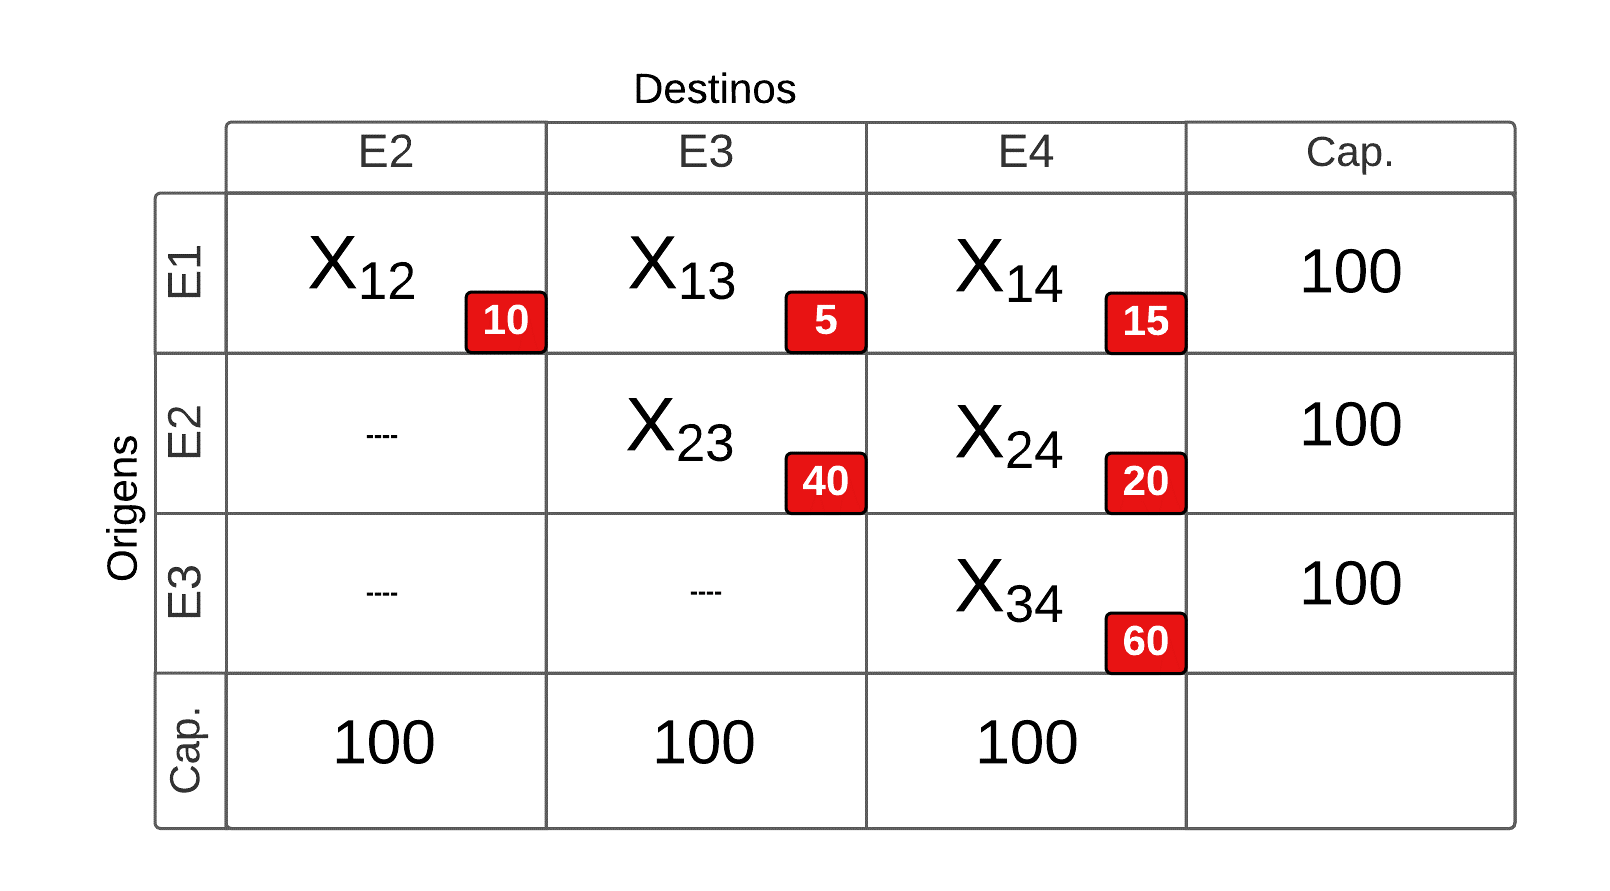
\includegraphics[scale=0.4]{img/fig3.png}
		\caption{Solução factível para o problema simplificado}
		% Fonte:~\cite{khaksar2013genetic}}
		\label{fig: fig3}
	\end{center}
\end{figure}

Observe que os valores das variáveis são os mesmos que foram mostrados na figura \ref{fig: fig3}. E ainda todas as restrições, tanto por linha quanto por coluna (por origens e por destinos), continuam sendo atendidas.

\begin{table}[h]
	\centering
	\small
	\begin{tabular}{p{2cm} p{9.5cm} p{3.2cm}}
		\toprule
		\textbf{Definição} & \textbf{Notação}                                                                     & \textbf{Domínio}                     \\ \midrule
		\multicolumn{3}{l}{\textbf{Conjuntos}}                                                                                                           \\ \midrule
		I                  & Conjunto de estações de Inicio                                                       &                                      \\
		J                  & Conjunto de estações de Destino                                                      &                                      \\
		K                  & Conjunto de Classes de Control                                                       &                                      \\
		T                  & Conjunto de Check-Points (Períodos)                                                  &                                      \\ \midrule
		\multicolumn{3}{l}{\textbf{Parâmetros}}                                                                                                          \\ \midrule
		n                  & Quantidade de estações                                                               &                                      \\
		Q                  & Capacidade do trem                                                                   &                                      \\
		P$_{ijk}$          & Preços  dos passagem com origem i, destino j e classe de control k                   & $i \in I, j \in J, k \in K$          \\
		D$_{ijkt}$         & Demanda  de passagem com origem i, destino j e classe de control k                   & $i \in I, j \in J, k \in K, t \in T$ \\ \midrule
		\multicolumn{3}{l}{\textbf{Variáveis de decisão}}                                                                                                \\ \midrule
		X$_{ijkt}$         & Quantidade de passagem atribuídos no tramo i,j com classe de control k no período t  & $i \in I, j \in J, k \in K, t \in T$ \\
		Y$_{ijkt}$         & Quantidade de passagem autorizados no tramo i,j com classe de control k no período t & $i \in I, j \in J, k \in K, t \in T$ \\ \bottomrule
	\end{tabular}
	\caption{Notação matemática}
	\label{Notacao}
\end{table}

\renewcommand{\baselinestretch}{0.5}

\begin{eqnarray}
	&& Max \quad Z = \sum_{i\in I} \sum_{j\in J} \sum_{k\in K} \sum_{t\in T} P_{ijk} X_{ijkt}                                             \label{eq: m2_ecu1}   \\
	&& \text{s.a.}  \notag                                                                                                                               \\
	&& \sum_{i\in I}\sum_{k\in K}\sum_{t\in T}X_{ijkt} \leq Q , \quad \forall j / j>1, i<j                                                \label{eq: m2_ecu2}   \\
	&& \sum_{j\in J}\sum_{k\in K}\sum_{t\in T}X_{ijkt} \leq Q , \quad \forall i / i<n, j>i                                                \label{eq: m2_ecu3}   \\
	&& Y_{ijkt} \geq X_{ijkt},  \quad \forall i,j,k,t/ i < j                                                                              \label{eq: m2_ecu4}   \\
	&& Y_{ijkt} \leq Y_{i,j,k+1,t},  \quad \forall i,j,k,t / i < j, k < \lVert K \rVert,  P_{ijk} \leq P_{i,j,k+1}                        \label{eq: m2_ecu5}   \\
	&& X_{ijkt} \leq D_{ijkt},  \quad \forall i,j,k,t/ i < j                                                                              \label{eq: m2_ecu6}   \\[15pt]
	&& X_{ijkt} \in \mathbb{Z}^+                                                                                                           \label{eq: m2_ecu7} \\
	&& Y_{ijkt} \in \mathbb{Z}^+                                                                                                           \label{eq: m2_ecu8}
\end{eqnarray}

Note que, na definição, não temos mais a variável de decisão de disponibilidade \(A_i\). Neste caso, a equação \ref{eq: m2_ecu1} representa a função objetivo, a restrição \ref{eq: m2_ecu2} garante que a quantidade total de assentos autorizados para cada destino seja a quantidade máxima de assentos do trem para todas as classes e todos os períodos. A restrição \ref{eq: m2_ecu3} garante que a quantidade de assentos autorizados para cada origem seja no máximo a capacidade do trem para todas as classes e todos os períodos. As restrições de \ref{eq: m2_ecu4} a \ref{eq: m2_ecu8} representam o mesmo que o primeiro modelo já exposto.